\paragraph{Dự báo so với SOH đo được.} Các hình dưới đây dùng cùng kịch bản: cell test không được đo dung lượng, lịch sử tới gốc là ước lượng, còn SOH đo được (chấm đen) chỉ dùng để chấm. Hình~\ref{fig:e22traj} cho một cell mỗi bộ, cell có sai số ở trung vị, với dự báo của ba mô hình học từ nhiều cell. Hình~\ref{fig:e22cells} cho ba cell mỗi bộ, chọn theo sai số của PINN-GBDT ở phân vị 25, 50 và 75\,\% trong số cell test của bộ, để thấy cả trường hợp dự báo tốt lẫn kém. Sai số trung bình trên phần đời còn lại của ba cell này là XJTU 13{,}1, 17{,}3, 24{,}0; TJU 3{,}7, 8{,}0, 14{,}3; MIT 7{,}0, 9{,}5, 12{,}3; HUST 11{,}7, 20{,}0, 42{,}4 ($\times10^{-3}$), và tỉ lệ chu kỳ có SOH đo nằm trong khoảng 90\,\% là XJTU 87\,\%, 100\,\%, 80\,\%; TJU 100\,\%, 99\,\%, 0\,\%; MIT 76\,\%, 100\,\%, 76\,\%; HUST 100\,\%, 100\,\%, 73\,\%. Ở cell phân vị 75\,\% của TJU, mức SOH ước lượng tại gốc đã cao hơn số đo 10{,}0$\times10^{-3}$; dự báo bắt đầu từ mức này nên lệch theo, và không chu kỳ nào có SOH đo nằm trong khoảng.

\begin{figure}[!htbp]\centering
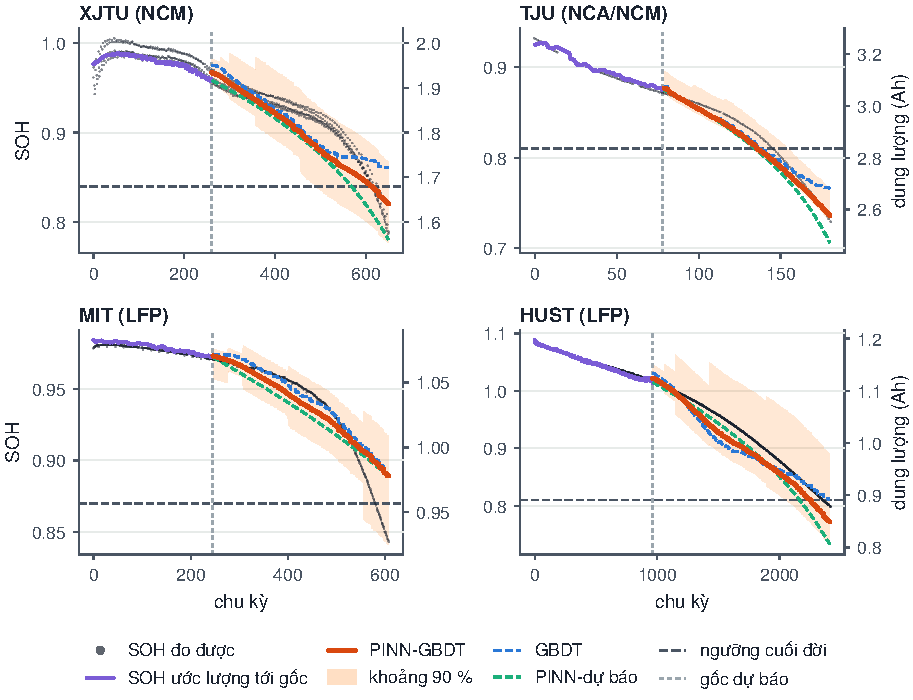
\includegraphics[width=\textwidth]{graphics/fig_e22_traj.pdf}
\caption[Dự báo cho một cell test mỗi bộ]{Dự báo cho một cell test mỗi bộ (lần lặp 0, gốc ở 40\,\% đời, cell có sai số của PINN-GBDT ở trung vị): SOH đo được (chấm), SOH ước lượng tới gốc, dự báo của GBDT, PINN-dự báo và PINN-GBDT kèm khoảng 90\,\%; trục phải là dung lượng (Ah).}\label{fig:e22traj}
\end{figure}

\begin{figure}[!htbp]\centering
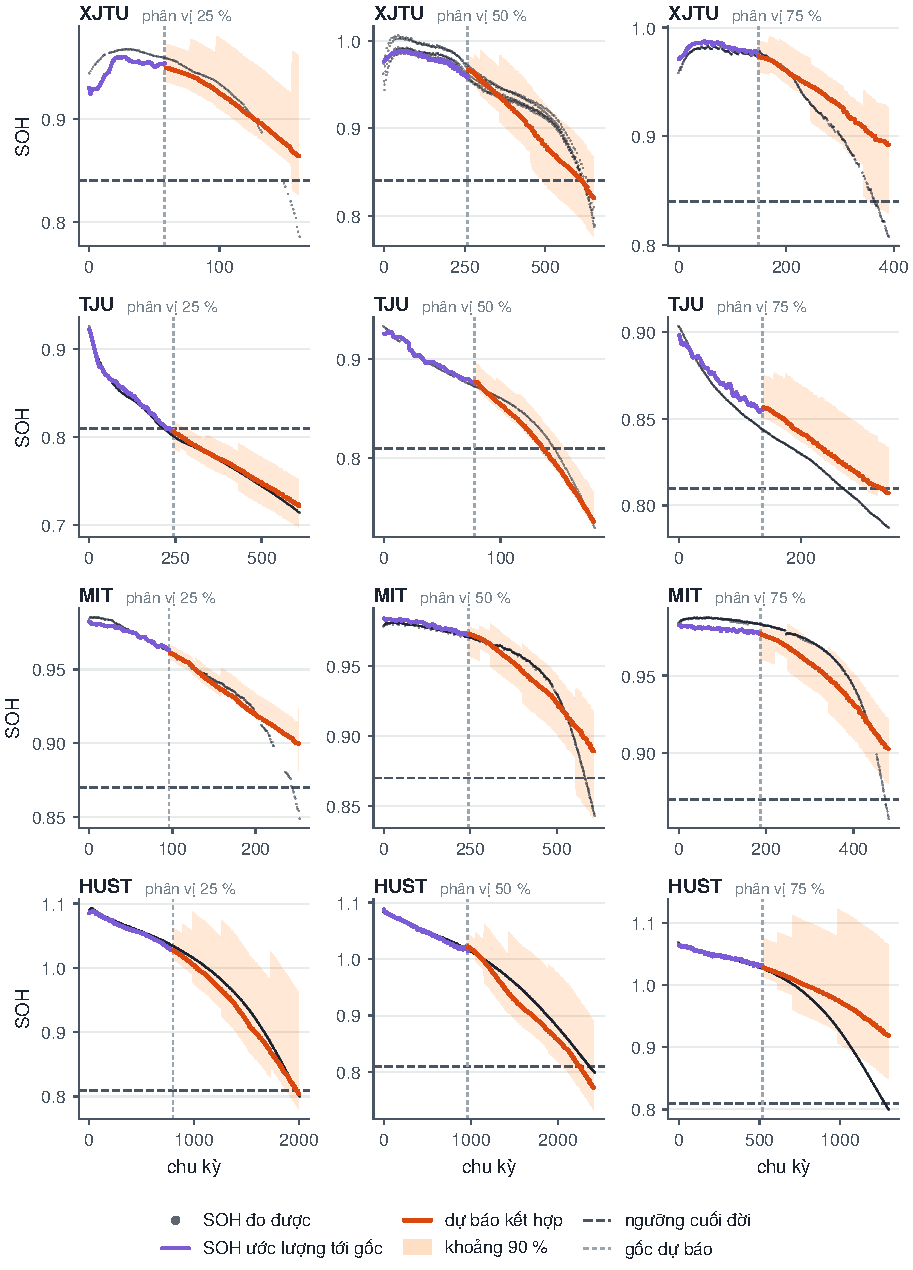
\includegraphics[width=\textwidth]{graphics/fig_e22_cells.pdf}
\caption[Dự báo so với SOH đo được, ba cell mỗi bộ]{Dự báo của PINN-GBDT so với SOH đo được cho ba cell test mỗi bộ, cell có sai số ở phân vị 25, 50 và 75\,\% của bộ (lần lặp 0, gốc ở 40\,\% đời, cell test không được đo dung lượng).}\label{fig:e22cells}
\end{figure}

\paragraph{Dự báo từ nhiều gốc.} Hình~\ref{fig:e22origins} giữ nguyên cell của Hình~\ref{fig:e22traj} và dự báo lại từ gốc ở 20, 40 và 60\,\% đời. Gốc muộn hơn thì lịch sử dài hơn và phần cần ngoại suy ngắn hơn, nhưng sai số cũng được chấm trên một đoạn khác, chỉ gồm phần đời còn lại sau gốc. Sai số trên phần đời còn lại, trung bình qua mọi cell và lần lặp, ở gốc 20, 40 và 60\,\% là XJTU 22{,}6, 23{,}0, 21{,}8; TJU 12{,}6, 11{,}5, 10{,}7; MIT 15{,}1, 11{,}7, 9{,}1; HUST 21{,}1, 28{,}6, 31{,}4 ($\times10^{-3}$): giảm dần theo gốc ở TJU và MIT, tăng dần ở HUST, gần như không đổi ở XJTU. Từ gốc 20\,\%, đường dự báo của XJTU và HUST trong hình đi ra mép dưới: khi $\lambda > 0$, nghiệm đóng~\eqref{eq:fcdrop} có điểm kỳ dị tại $h = 1/(\lambda a)$, nên ở tầm đủ dài PINN-dự báo rơi tới giới hạn dưới 0{,}40 của SOH và kéo PINN-GBDT xuống theo. Trên mọi cell và lần lặp, điều này xảy ra ở 2--5\,\% số quỹ đạo từ gốc 20\,\%, 1--3\,\% số quỹ đạo từ gốc 40\,\%, 0--3\,\% số quỹ đạo từ gốc 60\,\% (thấp nhất và cao nhất trong bốn bộ).

\begin{figure}[!htbp]\centering
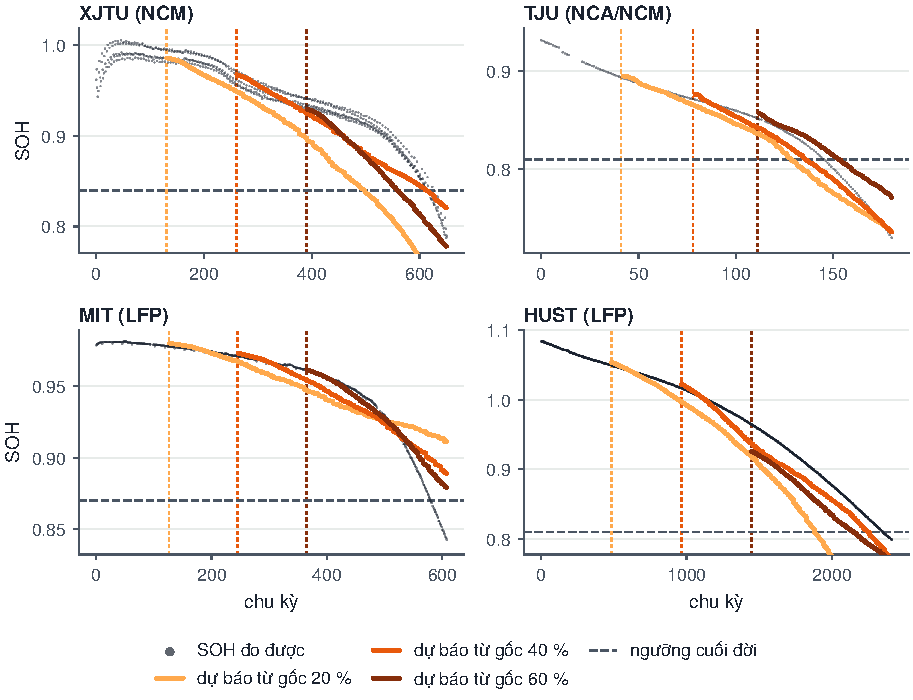
\includegraphics[width=\textwidth]{graphics/fig_e22_origins.pdf}
\caption[Dự báo từ ba gốc cho cùng một cell]{Dự báo của PINN-GBDT cho cùng cell của Hình~\ref{fig:e22traj} từ ba gốc ở 20, 40 và 60\,\% đời (đường chấm dọc), so với SOH đo được; trục SOH giữ theo khoảng của số đo, đường đi ra mép dưới là dự báo thấp hơn khung.}\label{fig:e22origins}
\end{figure}

\paragraph{SOH dự báo so với SOH đo ở ba tầm.} Hình~\ref{fig:e22parity} đặt SOH dự báo cạnh SOH đo được ở tầm $0{,}1L$, $0{,}25L$ và $0{,}5L$ cho mọi cell test và mọi gốc của lần lặp 0. Sai số tăng theo tầm ở cả bốn bộ (Bảng~\ref{tab:e22soh}), nên các điểm toả rộng dần khỏi đường chéo. Sai số có dấu trung bình (dự báo trừ số đo) ở ba tầm là XJTU −4{,}4, −9{,}8, −6{,}0; TJU −1{,}6, −3{,}8, −1{,}0; MIT −2{,}3, −3{,}6, −0{,}4; HUST −3{,}0, −4{,}0, −6{,}4 ($\times10^{-3}$), tức trung bình dự báo thấp hơn số đo ở cả ba tầm trên cả bốn bộ. Tỉ lệ số đo nằm trong khoảng 90\,\% ở ba tầm là XJTU 89\,\%, 90\,\%, 91\,\%; TJU 84\,\%, 81\,\%, 81\,\%; MIT 90\,\%, 96\,\%, 88\,\%; HUST 91\,\%, 88\,\%, 85\,\%. Số điểm có dự báo thấp hơn khung hình (vẽ bằng tam giác ở mép dưới) là XJTU 1 trên 403; TJU 5 trên 859; MIT 2 trên 920; HUST 12 trên 606.

\begin{figure}[!htbp]\centering
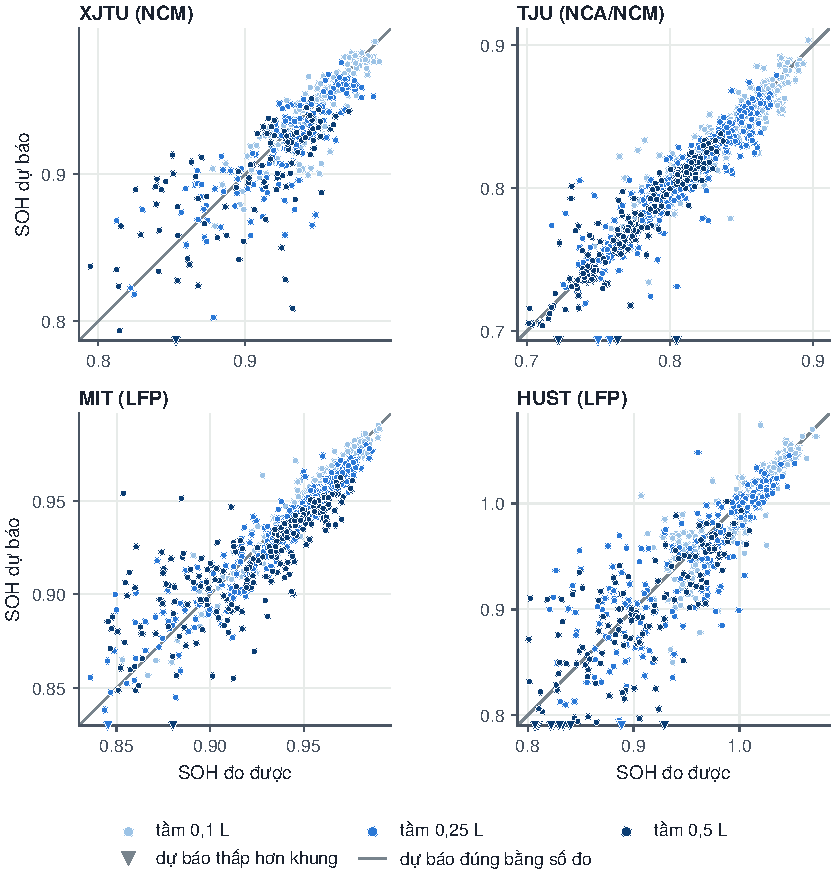
\includegraphics[width=\textwidth]{graphics/fig_e22_parity.pdf}
\caption[SOH dự báo so với SOH đo ở ba tầm]{SOH dự báo của PINN-GBDT so với SOH đo được ở ba tầm dự báo (lần lặp 0, mọi cell test, gốc ở 20, 40 và 60\,\% đời); đường chéo là dự báo đúng bằng số đo, tam giác ở mép dưới là dự báo thấp hơn khung.}\label{fig:e22parity}
\end{figure}

\paragraph{Sai số theo tầm và RUL.} Hình~\ref{fig:e22horizon} cho sai số của sáu mô hình theo tầm dự báo. Ở tầm $0{,}5L$, ba mô hình chỉ dựa vào lịch sử của chính cell đều kém PINN-GBDT trên cả bốn bộ; ở tầm ngắn $0{,}1L$, ít nhất một trong ba mô hình đó tốt hơn PINN-GBDT trên MIT và HUST (Bảng~\ref{tab:e22soh}). Hình~\ref{fig:e22rul} so RUL dự báo với RUL thực tại gốc ở 25, 50 và 75\,\% của chu kỳ cuối đời thật; tỉ lệ dự báo nằm trong $\pm20\,\%$ RUL thực là XJTU 38\,\%; TJU 65\,\%; MIT 48\,\%; HUST 52\,\%, và độ phủ của khoảng RUL 90\,\% là XJTU 70\,\%; TJU 84\,\%; MIT 67\,\%; HUST 65\,\%, thấp hơn mức đặt ra. Khoảng RUL được hiệu chỉnh trên ít cell validation (10\,\% số cell), trong khi sai số của một cell tương quan mạnh giữa các tầm, nên phân vị lấy từ vài cell hẹp hơn phân bố sai số của cell mới.

\begin{figure}[!htbp]\centering
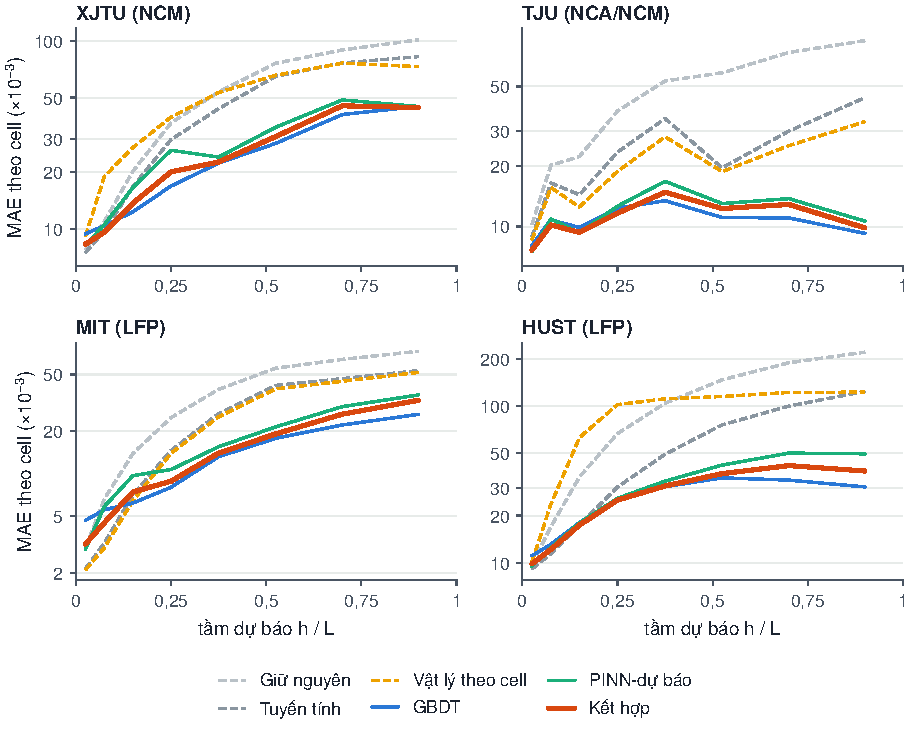
\includegraphics[width=\textwidth]{graphics/fig_e22_horizon.pdf}
\caption[Sai số dự báo theo tầm]{MAE theo cell của sáu mô hình theo tầm dự báo $h/L$ ($L$: trung vị số chu kỳ của bộ), kịch bản lịch sử ước lượng, mọi lần lặp và mọi gốc.}\label{fig:e22horizon}
\end{figure}

\begin{figure}[!htbp]\centering
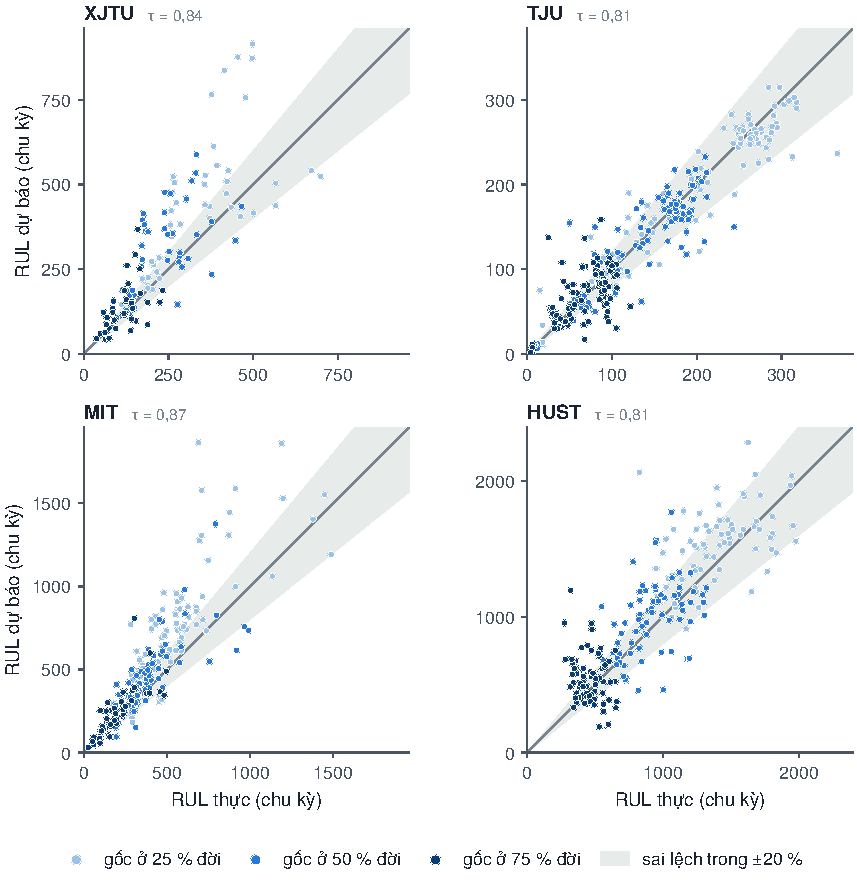
\includegraphics[width=\textwidth]{graphics/fig_e22_rul.pdf}
\caption[RUL dự báo so với RUL thực]{RUL dự báo của PINN-GBDT so với RUL thực, trung bình qua ba lần lặp, tại gốc ở 25, 50 và 75\,\% của chu kỳ cuối đời thật; dải xám là sai lệch trong $\pm20\,\%$, $\tau$ là ngưỡng cuối đời của bộ. Dự báo không chạm ngưỡng trong $3L$ chu kỳ được ghi là $3L$.}\label{fig:e22rul}
\end{figure}
